We have just seen one example in the previous section, where, by assuming that every loop in the program eventually terminates, the compiler is able to optimize certain loops and the code containing these loops. The fundamental logic used by the optimizer is always the same: first, we assume that the program does not exhibit UB. Then, we deduce the conditions that must be true in order for this assumption to hold and assume that these conditions are indeed always true. Finally, any optimization that is valid under such assumptions may proceed. The code generated by the optimizer will do something if the assumptions are violated, but we have no way of knowing what it will be (beyond the already mentioned restrictions that it's still the same computer executing some sequence of instructions).

Almost every case of UB documented in the standard can be converted into an example of a possible optimization (whether a particular compiler takes advantage of this is a different matter). We are going to see several more examples now.

As we have already mentioned, the result of overflowing a signed integer is undefined. The compiler is allowed to assume that this never happens and that incrementing a signed integer by a positive number always results in a greater integer. Do the compilers actually perform this optimization? Let's find out. Compare these two functions, f() and g():

\hspace*{\fill} \\ %插入空行
\noindent
\textbf{03\_int\_overflow.C}
\begin{lstlisting}[style=styleCXX]
bool f(int i) { return i + 1 > i; }
bool g(int i) { return true; }
\end{lstlisting}

Within the realm of well-defined behavior, these functions are identical. We could try to benchmark them to determine whether the compiler optimizes away the entire expression in f() but, as we have seen in the previous chapter, there is a more reliable way. If both functions generate the same machine code, they are definitely identical. 

\hspace*{\fill} \\ %插入空行
\begin{center}
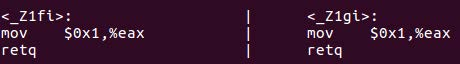
\includegraphics[width=0.9\textwidth]{content/3/chapter11/images/1.jpg}\\
Figure 11.1 – x86 assembly output generated by GCC9 for the f() (left) and g() (right) functions
\end{center}

In Figure 11.1, we can see that with optimization turned on, GCC indeed generates the same code for both functions (so does Clang). The names of the functions that show up in the assembly are so-called mangled names: since C++ allows functions with different parameter lists to have the same name, it has to generate a unique name for each of suchfunctions. It does so by encoding the types of all parameters into the name that is actually used in the object code.

If you want to validate that this code indeed does not have any trace of the ?: operator, the easiest way is to compare the f() function with a function that does the same computation using unsigned integers. Refer to the following code:

\hspace*{\fill} \\ %插入空行
\noindent
\textbf{03\_int\_overflow.C}
\begin{lstlisting}[style=styleCXX]
bool f(int i) { return i + 1 > i; }
bool h(unsigned int i) { return i + 1 > i; }
\end{lstlisting}

Overflow of unsigned integers is well defined, and it is, in general, not true that i + 1 is always greater than i. 

\hspace*{\fill} \\ %插入空行
\begin{center}
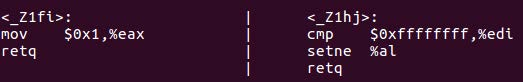
\includegraphics[width=0.9\textwidth]{content/3/chapter11/images/2.jpg}\\
Figure 11.2 – X86 assembly output generated by GCC9 for the f() (left) and h() (right) functions
\end{center}

The h() function produces different code, and you can guess that the cmp instruction does a comparison even if you are not fluent in X86 assembly. On the left, the function f() loads the constant value of 0x1, otherwise known as true for Booleans, into the register EAX that is used to return the result. 

This example also demonstrates the danger of trying to reason about UB or treat it as implementation-defined: if you were to say that the program will do some kind of addition for the integers and if it overflows, the particular hardware would do whatever it does, and you would be very wrong. A compiler may, and some do, generate code with no increment instructions at all.

We now, finally, have enough knowledge to fully elucidate the mystery whose seeds were planted all the way at the beginning of the book, in Chapter 2, Performance Measurements. In that chapter, we observed an unexpected performance difference between two almost identical implementations of the same function. The function's job was to compare two strings, character by character, and return true if the first string is lexicographically greater. This was our most compact implementation:

\hspace*{\fill} \\ %插入空行
\noindent
\textbf{04a\_compare1.C}
\begin{lstlisting}[style=styleCXX]
bool compare1(const char* s1, const char* s2) {
	if (s1 == s2) return false;
	for (unsigned int i1 = 0, i2 = 0;; ++i1, ++i2) {
		if (s1[i1] != s2[i2]) return s1[i1] > s2[i2];
	}
}
\end{lstlisting}

This function was used to sort strings, so the benchmark measured the time of sorting a particular input set of strings:

\hspace*{\fill} \\ %插入空行
\begin{center}
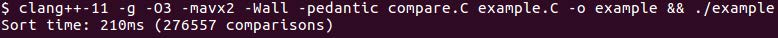
\includegraphics[width=0.9\textwidth]{content/3/chapter11/images/3.jpg}\\
Figure 11.3 – Sorting benchmark using the compare1() function for string comparison
\end{center}

The comparison implementation is as compact as it gets; there is nothing unnecessary in this code. However, the surprising result was that this was one of the worst-performing versions of the code. The best-performing version was almost the same:

\hspace*{\fill} \\ %插入空行
\noindent
\textbf{04b\_compare2.C}
\begin{lstlisting}[style=styleCXX]
bool compare2(const char* s1, const char* s2) {
	if (s1 == s2) return false;
	for (int i1 = 0, i2 = 0;; ++i1, ++i2) {
		if (s1[i1] != s2[i2]) return s1[i1] > s2[i2];
	}
}
\end{lstlisting}

The only difference is the type of the loop variable: unsigned int in compare1() versus int in compare2(). Since the indices are never negative, this should make no difference whatsoever, but it does:

\hspace*{\fill} \\ %插入空行
\begin{center}
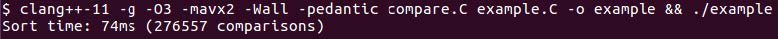
\includegraphics[width=0.9\textwidth]{content/3/chapter11/images/4.jpg}\\
Figure 11.4 – Sorting benchmark using the compare2() function for string comparison
\end{center}

The reason for this significant performance difference again has to do with UB. To understand what is going on, we will have to examine the assembly code again. Figure 11.5 shows the code generated by GCC for both functions (only the most relevant part, the string comparison loop, is shown):

\hspace*{\fill} \\ %插入空行
\begin{center}
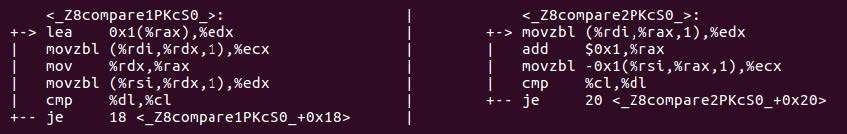
\includegraphics[width=0.9\textwidth]{content/3/chapter11/images/5.jpg}\\
Figure 11.5 – X86 assembly generated for the compare1() (left) and compare2() (right) functions
\end{center}

The code looks pretty similar, with one exception: on the right (compare2()), you can see the add instruction, which is used to increment the loop index by 1 (the compiler optimized the code by replacing two loop variables with just one). On the left, there is nothing that looks like an addition or increment. Instead, there is the lea instruction, which stands for Load and Extend Address, but is used here to increment the index variable by 1 (the same optimization is done; there is only one loop variable). 

With everything you have learned up to now, you should be able to guess why the compiler has to generate different code: while the programmer expects the index to never overflow, the compiler, in general, cannot make this assumption. Note that both versions use 32-bit integers, but the code is generated for a 64-bit machine. If a 32-bit signed int overflows, the result is undefined, so in this case, the compiler does make the assumption that the overflow never happens. If the operation does not overflow, the add instruction produces the correct result. For unsigned int, the compiler has to allow for the possibility of the overflow: incrementing UINT\_MAX should give 0. It turns out that the add instruction on x86-64 does not have these semantics. Instead, it extends the result to become a 64-bit integer. The best option for 32-bit unsigned integer arithmetic on X86 is the lea instruction; it does the job but is much slower.

This example demonstrates how, by reasoning backward from the assumption that the program is well defined and UB never happens, the compiler can enable a very effective optimization that ends up making the entire sort operation several times faster.

Now that we understand what is going on in our code, we can explain the behavior of several other versions of the code. First of all, using 64-bit integers, signed or unsigned, will give us the same fast performance as the 32-bit signed integers: in all cases, the compiler will use add (for 64-bit unsigned values, it does have the correct overflow semantics). Second, if the maximum index, or the string length, is used, the compiler will deduce that the index cannot overflow:

\begin{lstlisting}[style=styleCXX]
bool compare1(const char* s1, const char* s2,
unsigned int len) {
	if (s1 == s2) return false;
	for (unsigned int i1 = 0, i2 = 0; i1 < len; ++i1, ++i2) {
		if (s1[i1] != s2[i2]) return s1[i1] > s2[i2];
	}
	return false;
}
\end{lstlisting}

The unnecessary comparison with the length makes this version slightly slower than the best variant. The most reliable way to avoid accidentally running into this problem is to always use signed loop variables or use the unsigned integer of the size native to the hardware (so, avoid doing unsigned int math on 64-bit processors unless you really need it).

We can construct similar demonstrations using almost any other situation described as undefined behavior in the standard (although there is no guarantee that a particular compiler will take advantage of a possible optimization). Here is one more example that uses pointer dereference:

\hspace*{\fill} \\ %插入空行
\noindent
\textbf{06a\_null.C}
\begin{lstlisting}[style=styleCXX]
int f(int* p) {
	++(*p);
	return p ? *p : 0; // Optimized to: return *p
}
\end{lstlisting}

This is a simplification of a pretty common situation where the programmer has coded pointer checks to protect against null pointers, but hasn't done so everywhere. The second line (the increment) is UB if the input argument is a null pointer. This means the entire program's behavior is undefined, so the compiler can assume it never happens. Examination of the assembly code shows that, indeed, the comparison in the third line is eliminated:

\hspace*{\fill} \\ %插入空行
\begin{center}
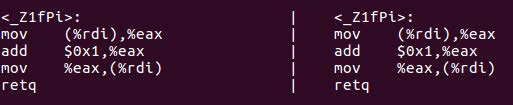
\includegraphics[width=0.9\textwidth]{content/3/chapter11/images/6.jpg}\\
Figure 11.6 – X86 assembly generated for the f() function with (left) and without (right) the ?: operator
\end{center}

The same happens if we do the pointer check first:

\hspace*{\fill} \\ %插入空行
\noindent
\textbf{07a\_null.C}
\begin{lstlisting}[style=styleCXX]
int f(int* p) {
	if (p) ++(*p);
	return *p;
}
\end{lstlisting}

Again, an examination of the assembly code will show that the pointer comparison is eliminated, even though the program behavior up to this point is well defined. The reasoning is the same: if the pointer p is not null, the comparison is redundant and can be omitted. If p is null, the behavior of the program is undefined, which means the compiler can do whatever it wants, and what it wants is to omit the comparison. The end result is, whether p is null or not, the comparison can be eliminated.

In the last chapter, when we studied compiler optimizations, we devoted a great deal of time to the analysis of what optimizations are possible because the compiler can prove that they are safe. We are going to revisit this issue because, first, it is absolutely essential for understanding compiler optimizations, and second, there is a connection with UB. We have just seen that when the compiler deduces some information from a particular statement (such as p is non-null deduced from the return statement), that knowledge is used to optimize not just following but also preceding code. The limitations on propagating such knowledge arise from what else the compiler can prove with certainty. To demonstrate, let's modify the previous example slightly:

\hspace*{\fill} \\ %插入空行
\noindent
\textbf{08a\_null.C}
\begin{lstlisting}[style=styleCXX]
extern void g();
int f(int* p) {
	if (p) g();
	return *p;
}
\end{lstlisting}

In this case, the compiler will not eliminate the pointer check, which can be seen in the produced assembly code:

\hspace*{\fill} \\ %插入空行
\begin{center}
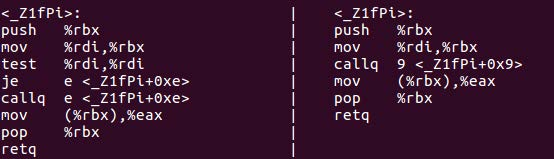
\includegraphics[width=0.9\textwidth]{content/3/chapter11/images/7.jpg}\\
Figure 11.7 – X86 assembly generated for the f() function with (left) and without (right) the pointer check
\end{center}

The test instruction does a comparison with null (zero) and is followed by a conditional jump – this is what the if statement looks like in assembly. 

Why didn't the compiler optimize away the check? To answer this question, you have to figure out under what conditions this optimization would have changed the well-defined behavior of the program.

The following two things are needed to make the optimization invalid:

\begin{itemize}
\item 
First, the g() function must know whether the pointer p is null. This is possible: for example, p could also be stored in a global variable by the caller of f(). 

\item 
Second, if p is null, the return statement must not be executed. This is also possible: g() may throw an exception if p is null. 
\end{itemize}

For our final example of C++ optimizations that are strongly related to UB, we are going to look at something very different: the effect of the const keyword on the optimization. Again, this will teach us just as much about why the compiler cannot optimize certain code as it does with successful optimizations. We are going to start with the code fragment we saw earlier:

\begin{lstlisting}[style=styleCXX]
bool f(int x) { return x + 1 > x; }
\end{lstlisting}

An optimizing compiler will, as we have seen, eliminate all the code from this function and replace it with return true. Now we will make the function do some more work:

\begin{lstlisting}[style=styleCXX]
void g(int y);
bool f(int x) {
	int y = x + 1;
	g(y);
	return y > x;
}
\end{lstlisting}

The same optimization is, of course, possible, since the code can be rewritten as follows:

\begin{lstlisting}[style=styleCXX]
void g(int y);
bool f(int x) {
	g(x + 1);
	return x + 1 > x;
}
\end{lstlisting}

The call to g() must be made, but the function still returns true: the comparison cannot produce anything else without lapsing into undefined behavior. Again, most compilers will do this optimization. We can confirm this by comparing the assembly generated from our original code with that generated from the fully hand-optimized code:

\begin{lstlisting}[style=styleCXX]
void g(int y);
bool f(int x) {
	g(x + 1);
	return true;
}
\end{lstlisting}

The only reason the optimization is possible is because the g() function does not change its argument. In the same code, if g() takes the argument by reference, the optimization is no longer possible:

\begin{lstlisting}[style=styleCXX]
void g(int& y);
bool f(int x) {
	int y = x + 1;
	g(y);
	return y > x;
}
\end{lstlisting}

Now the g() function could change the value of y, so the comparison has to be made every time. If the intent for the function g() is not to change its arguments, we could, of course, just pass them by value (as we have already seen). The other option is to pass by const reference; while there is no reason to do so for small types, such as integers, template code often generates such functions. In this case, our code looks like this:

\hspace*{\fill} \\ %插入空行
\noindent
\textbf{10\_const.C}
\begin{lstlisting}[style=styleCXX]
void g(const int& y);
bool f(int x) {
	int y = x + 1;
	g(y);
	return y > x;
}
\end{lstlisting}

A quick examination of the assembler shows that the return statement is not optimized: it still does the comparison. Of course, the fact that a particular compiler does not do a certain optimization proves nothing: no optimizer is perfect. But in this case, there is a reason for it. Despite what the code says, the C++ Standard does not guarantee that the g() function does not change its argument! Here is an entirely Standard-compliant  implementation that elucidates the issue:

\begin{lstlisting}[style=styleCXX]
void g(const int& y) { ++const_cast<int&>(y); }
bool f(int x) {
	int y = x + 1;
	g(y);
	return y > x;
}
\end{lstlisting}

Yes, a function is allowed to cast away const. The result is well defined and is specified in the standard (which does not make it a good code, just a valid one). There is one exception, however: casting away const from an object that was declared const at the point of its creation is UB. To illustrate, this is well defined (but ill-advised):

\begin{lstlisting}[style=styleCXX]
int x = 0;
const int& y = x;
const_cast<int&>(y) = 1;
\end{lstlisting}

This is UB:

\begin{lstlisting}[style=styleCXX]
const int x = 0;
const int& y = x;
const_cast<int&>(y) = 1;
\end{lstlisting}

We can try to take advantage of this by declaring the intermediate variable y as const:

\begin{lstlisting}[style=styleCXX]
void g(const int& y);
bool f(int x) {
	const int y = x + 1;
	g(y);
	return y > x;
}
\end{lstlisting}

Now the compiler can assume that the function always returns true: the only way to change that is to invoke UB, and the compiler is not required to condone UB. At the time of the writing of this book, we are not aware of any compiler that actually does this optimization.

With this in mind, what can be recommended with regard to the use of const to promote optimization?

\begin{itemize}
\item 
If a value is not changing, declare it as const. While correctness is the main benefit, this does enable some optimizations, especially when the compiler can propagate the const by evaluating expressions at compile time.

\item 
Even better for the optimization, if the value is known at compile-time, declare it constexpr.

\item 
Passing parameters by const reference to functions does next to nothing for optimization since the compiler has to assume that the function may cast away const (if the function is inlined, the compiler knows exactly what's going on, but then it doesn't matter how the parameters are declared). On the other hand, this is the only way you can pass a const object to a function, so yes, declare references to be const whenever possible (the more important result is the clarity of the intent).

\item 
For small types, pass-by-value can be more efficient than pass-by-reference (this does not apply to inlined functions). This is difficult to reconcile with generic functions generated by templates (don't assume that the templates are always inlined; large template functions often aren't). There are ways to force pass-by-value for specific types, but they make your template code much more cumbersome. Never start by writing such code; do it only if the measurements show that, for a particular piece of code, the effort is justified.

\end{itemize}

We have explored in detail how UB in C++ affects the optimization of C++ code. It is now time to turn the tables and learn how to take advantage of UB in your own programs.
























